\documentclass[conference,a4paper]{IEEEtran}
\IEEEoverridecommandlockouts
% The preceding line is only needed to identify funding in the first footnote. If that is unneeded, please comment it out.
%Template version as of 6/27/2024

\usepackage{cite}
\usepackage{amsmath,amssymb,amsfonts}
\usepackage{algorithmic}
\usepackage{graphicx}

\usepackage{textcomp}
\usepackage{tikz}
\usepackage{booktabs}
\usepackage{xcolor}
\usepackage{hyperref}
\usepackage{array}
\usepackage{tabularx}
\usepackage{amssymb} 


\def\BibTeX{{\rm B\kern-.05em{\sc i\kern-.025em b}\kern-.08em
    T\kern-.1667em\lower.7ex\hbox{E}\kern-.125emX}}
\begin{document}

% Custom figure command: pass filename and caption
\newcommand{\cfigure}[2]{%
  \begin{figure}[h]
    \centering
    \includegraphics[width=\linewidth]{figures/#1.png}%
    \caption{#2}%
    \label{fig:#1}%
  \end{figure}%

}
\title{Summary of Potential of artificial intelligence in reducing energy and carbon emissions of commercial buildings at scale}

\author{Dwayne Mark Acosta (300665276) \\ Mohamed Amine Benaziza (300684553) \\ David Franz (300360491) \\ Ray Marange (300671115) \\ James Thompson (300680096)\\
\textit{Victoria University of Wellington}\\}
\date{\today}

\maketitle

\section*{Introduction}
Climate change is accelerating, and buildings are a major contributor, responsible for 39\% of U.S. primary energy use. With urbanization surging and building stock/demand expected to double by 2060, improving building efficiency is no longer optional but urgent.
While AI has transformed industries such as healthcare and finance, its potential in building energy efficiency remains underexplored. AI demonstrates significant potential to reduce costs, enhance benefits, and improve safety across the building lifecycle. This study \cite{dingPotentialArtificialIntelligence2024} investigates how AI can reduce energy consumption and carbon emissions in medium-sized office buildings, offering a scalable framework that could be applied globally.
We will explore four key areas: \textbf{Results}, \textbf{Discussion}, \textbf{Methods}, and \textbf{Takeaways \& Reflections}. The study focuses on medium-sized offices, and the results can be extrapolated to offices of any size.


\section*{AI's impact on energy and emission reductions}

According to the 2012 U.S. Energy Information Association (EIA) survey \cite{USEIACommercial}, office buildings have the highest energy consumption among commercial types (20\%), with a median energy use intensity (EUI) of 167~kWh/m\textsuperscript{2} (EUI\textsubscript{base}). In contrast, 67 verified low-energy office buildings reported a median EUI of 57~kWh/m\textsuperscript{2} (EUI\textsubscript{HEEB}). The difference between the baseline and best practice energy performance yields a technical energy efficiency saving (TEES) of 110~kWh/m\textsuperscript{2}. TEES can be improved in four categories: equipment, occupancy influence, control and operation, and design and construction.

This study focuses on medium office buildings, which comprise 70\% of total office energy use. The Department of Energy's (DOE) EnergyPlus tool, defined by ASHRAE Standard 90.1 \cite{ASHRAEANSIASHRAE}, was used to simulate the annual building energy consumption of medium office buildings across four climate zones (1A, 3B, 4A, 5A) using representative U.S. cities. Both electricity and natural gas use were considered, with gas assumed to supply hot water and heating. 

To estimate the TEES, a set of 24 improvement cases was developed by varying key design parameters. These include 9 cases for equipment efficiency, 9 for design and construction, and 6 for occupancy-related behavior and control. The cases, based on conservative assumptions, are summarized in Table~\ref{tab:all-cases}, and their contributions to total annual energy savings across different climate zones are illustrated in Figure~\ref{fig:category-breakdown}. The results represent the maximum technical potential achievable through simulation, achieving these savings in practice may require substantial effort throughout the building lifecycle. AI technologies such as fault detection, smart sensors, robotic construction and others can help automate and streamline this process at lower cost and reduced labor.

\subsection*{Thoughts and takeaways}
Although simulation results suggest that TEES across the four categories can range from 6\% to 27\%, the paper assumes highly optimized performance which is often difficult to achieve in practice due to real-world constraints. While AI technologies may support these optimizations, their effectiveness is not guaranteed and remains highly dependent on a wide range of factors including data quality, user adoption, and integration with current systems.

\section*{AI's reduces emissions of buildings}

This section is about modeling the energy use and emissions in buildings in existing buildings (which can be retrofitted with more energy efficient options later), construction of new buildings, and overall impact over these buildings' lifetimes.

Using the results from the previous section as input parameters, a variety of complex simulations are produced by to understand the short and long term impact of these buildings.

\subsection*{Primary focus of modeling}

The paper primarily focuses on two ways that AI can increase energy efficiency and reduce the emissions of buildings.

\begin{enumerate}
    \item By helping scale up the technologies and speed adoption by reducing the construction and labor costs;
    \item By helping reduce emissions in ongoing maintenance and any new construction over the entire building's lifetime.
\end{enumerate}

\subsection*{Scenarios simulated}
The paper uses the results gained from the previous section to \textbf{simulate six scenarios}. The data is used to estimate parameters for use with complex simulation software to attempt to model the potential lifetime impact on emissions.
\begin{enumerate}
    \item Frozen with current building efficiency;
    \item Business as usual without AI;
    \item Business as usual with AI;
    \item Three policy-driven scenarios promoting high-efficiency energy buildings and net-zero energy buildings, and other policy implementation to achieve zero emissions by 2050.
\end{enumerate}


\subsection*{Simulation results}
The results of the simulation are shown below.

\begin{table}
\centering
\begin{tabular}{|c|c|c|}
\hline
\textbf{Scenario} & \textbf{Energy Use (kWh/m$^2$)} & \textbf{CO$_2$ Emissions (kg/m$^2$)} \\
\hline 
Baseline & 200 & 50 \\
\hline
AI Optimized & 150 & 30 \\
\hline
\end{tabular}
\caption{Energy use and CO$_2$ emissions for different scenarios.}
\label{tab:energy-emissions}
\end{table}

Table \ref{tab:energy-emissions} shows the energy use and CO$_2$ emissions for different scenarios.

\cfigure{cool-figure}{Different energy use scenarios.}

\subsection*{Key insight}

\textit{“The scenario with AI leads to a higher market share of HEEBs and NZEBs over time compared with the scenario without AI. This trend continues until the market share of net NZEBs reaches its maximum share.”}

The paper asserts that using AI in the ways that they propose always leads to a higher market share of efficient buildings. 

\subsection*{Thoughts and takeaways}
The paper examines various scenarios with some amount of estimation for unknowns, so each individual simulation is unlikely to be exactly right. However, the fact that all scenarios trend in a downward direction for energy use and $CO_2$ emissions suggest it is highly likely that AI would have some impact on building emissions, but the current lack of data leading to necessary estimation means that the current degree of this impact is still unclear.


\section*{Discussion}

The study uses a combination of engineering and energy-simulation approaches, rather than focusing on a single AI technology, to estimate how AI can boost building energy efficiency and reduce carbon emissions. While the analysis centers on a medium-sized office building, the methodology is adaptable to other commercial building types with appropriate adjustments.

AI enables data-driven modeling, which can tailor solutions to specific buildings and lower costs. This accelerates the adoption of high-efficiency and net-zero-energy buildings (HEEBs and NZEBs). The paper also notes that advanced control models, such as deep learning and reinforcement learning, could further improve accuracy in future work.

The paper evaluates the theoretical maximum savings achievable over a building’s lifetime. It highlights that different climate zones offer varying saving potentials, but in all cases, AI can help buildings achieve these potentials at lower costs. They have quantified these numbers for the medium office building example.
\begin{itemize}
    \item By 2050, AI adoption alone is projected to reduce energy use and CO$_2$ emissions by approximately 8\% compared to the “business as usual” (BAU) scenario.
    \item When compared to a policy-only scenario, AI provides an additional 19\% in savings.
    \item The combination of AI, strong efficiency policies, and low-emission power generation (LEPG) could result in up to 40\% less energy use and 90\% less CO$_2$ emissions than BAU.
\end{itemize}

\subsection*{Thoughts and takeaways}
\begin{enumerate}
    \item \textbf{Limitations:} The results depend on assumptions about cost declines and adoption rates. Additionally, the methodology has not yet been tested on other building types, which may limit the generalizability of the findings.
    \item \textbf{Paper’s Goal:} The main contribution is not a new algorithm, but rather the demonstration that AI can make existing high-efficiency designs more affordable, thereby unlocking a larger market share for these technologies.
    \item \textbf{Role of Policy:} On its own, AI delivers modest (single-digit) gains. The substantial reductions of 40\% in energy use and 90\% in CO$_2$ emissions are only achieved when AI is combined with LEPG and clear regulatory policies.
    \item \textbf{Scalability:} Expanding these results to other sectors will require further investigation and the development of skilled facility management teams.
\end{enumerate}

\section*{Methods}

This paper makes a few claims around the potential energy use reduction that can happen now and as different future scenarios play out. For them to calculate the potential savings you need models and numbers to put in the models.

\subsection*{Energy saving potentials}

The first model they use is particularly simple which is just the summation of the potential saving across the four areas of the building mutiplied by the base energy use. The values of potential savings are calculated using the building simulations and other literature. This is the strongest and most reliable model they use.

\subsection*{Market share of HEEB and NZEB in the future}

The next models they use are for studying how different scenarios will play out. The first model is a discrete choice model that calculates what share of a population will take a particular choice. The share is calculated as simply a ratio of its availability and utility and the sum of other choices availability and utility Eq \ref{eq:share}. The utility of each type of building is calculated by using a future discounted sum of the net benefit at each time Eq \ref{eq:utility}.

The last model is used to calculate the cost of the different buildings. Specifically high energy efficient buildings (HEEB) and net zero energy buildings (NZEB). Having a look at Eq \ref{eq:cost} there are three parameters they have set. Firstly is how much more expensive NZEB are then HEEB buildings. Secondly is how quickly this premium will decrease autonomously and due to policy. Lastly is how much AI will decrease the premium.

The cost premium of NZEB buildings over regular buildings is 13-19\% when looking at the four climate zones with HEEB buildings being about 5\% cheaper than NZEB. These figures are estimated from construction cost data. The amount the premium will decrease autonomously and due to AI are simply estimated by the authors. Furthermore AI is simply assumed to decrease the cost premium by an extra 10\% overall without any justification.

The last part to the model of the market share is availability, while not stating explicitly how it is done the availability is a combination of retrofitting old buildings and maximum amount allowed in the market. The NZEB buildings have a market share of 59\%-79\% depending on the scenario. With an estimated annual retrofit of 0.5\%-3.5\% depending on scenario. These values have been estimated by the author with some being adapted from previous studies. In this study they assume AI can increase the maximum share by 2\%.

\subsection*{Thoughts and takeaways}
In this study they have used simple reasonable models which makes their method accessible. However the models are sensitive to the parameters you choose to use and in this case many of their parameter choices are lacking adequate support. As a consequence their conclusions are not as strong as they could be, and future forecasted numbers are ideals not rigorous predictions. \footnote{Thane Ruthenis (prominent commentator of AI forums) comment says it best \cite{ruthenisDeepCritiqueAI2025}}. These model are a good framework but more forecasting work is needed to understand the future effect of AI and provide more supported parameters to the models.


\begin{align}
  \text{share}_{i,t} &= \frac{a_{i,t}\exp{(u_{i,t})}}{\sum_{i=0}^{N-1}a_{i,t}\exp{(u_{i,t})}}\label{eq:share} \\
  u_{i,t} &= \sum_{t}^{\text{max}_t}d_t(B_{i,t}-C_{i,t}) \label{eq:utility}\\
  C_{i,t} &= CC_0+ \nabla CC_k\times(1-\alpha_{k,t}-\xi_{k,t}) +\nonumber\\& DC_0+\nabla DC_k+(1-\beta_{k,t}-\zeta_{k,t}) \label{eq:cost}
\end{align}

\bibliographystyle{IEEEtran}
\bibliography{references}

\appendix


    
\begin{table}[h]
  \centering
  \caption{Summary of Energy Efficiency Improvement Cases Across All Categories}
  \label{tab:all-cases}
  \begin{tabularx}{\linewidth}{|c|>{\raggedright\arraybackslash}X|>{\raggedright\arraybackslash}X|}
  \hline
  \textbf{Case} & \textbf{Improvements} & \textbf{Adjustments} \\
  \hline
  \multicolumn{3}{|c|}{\textbf{Equipment Efficiency Improvements}} \\
  \hline
  E1 & HVAC – Cooling & +20\% \\
  E2 & HVAC – Heating & +12\% \\
  E3 & HVAC – Cases E1 and E2 & +20\%, +12\% \\
  E4 & Lighting – Power density (LPD) & -15\% \\
  E5 & Lighting – Power density (LPD) & -21\% \\
  E6 & Equipment – Power density (EPD) & -10\% \\
  E7 & Equipment – Power density (EPD) & -20\% \\
  E8 & Combined – Cases E1–E7 & \\
  E9 & Case E8 + Heat Pump for space heating & \\
  \hline
  \multicolumn{3}{|c|}{\textbf{Design and Construction Improvements}} \\
  \hline
  D1 & Orientation & East (90° rotation) \\
  D2 & Orientation & South (180° rotation) \\
  D3 & Orientation & West (270° rotation) \\
  D4 & Envelope (walls, slabs, roofs, windows) & High insulation \\
  D5 & Envelope (walls, slabs, roofs, windows) & Increased infiltration (~60\%) \\
  D6 & Window-to-wall ratio (WWR) & Variation 1 \\
  D7 & Window-to-wall ratio (WWR) & Variation 2 \\
  D8 & Window-to-wall ratio (WWR) & Variation 3 \\
  D9 & Combined – Orientation, insulation, WWR & \\
  \hline
  \multicolumn{3}{|c|}{\textbf{Occupant Behavior and Control Improvements}} \\
  \hline
  B1 & Ventilation control & Open/close windows \\
  B2 & Lighting use & Switch on/off lights \\
  B3 & Electricity consumption & Turn off plug loads \\
  B4 & Lighting use & Dim lights \\
  B5 & HVAC & Turn on/off HVAC systems \\
  B6 & Thermostat & Adjust thermostat settings \\
  \hline
  \multicolumn{3}{|c|}{
    \begin{tabular}[c]{@{}c@{}}
      \textbf{Energy savings:} \\
      Equipment = 11.5--17.3\% \\
      Design and Construction = 5.9--9.1\% \\
      Occupant Behavior and Control and Operation = 15--20\%
    \end{tabular}
  } \\
  \hline
  \end{tabularx}
\end{table}

        
\begin{figure}[h]
  \centering
  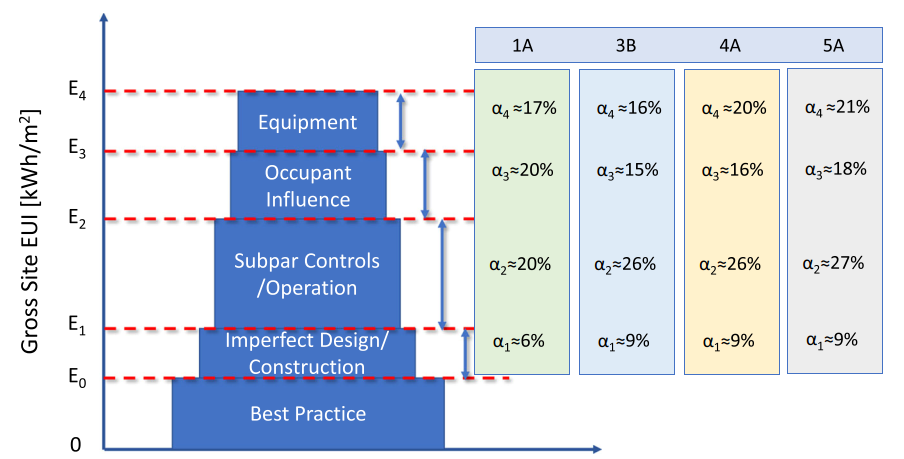
\includegraphics[width=\linewidth]{figures/Integrated technical building energy-saving potential of a typical medium office building in the United States.png}
  \caption{Integrated building energy-saving breakdown by category and climate zone.}
  \label{fig:category-breakdown}
\end{figure}

  

\end{document}
